\subsection{Análise trimestral}
Agregando os valores para períodos trimestrais conseguimos chegar aos dados presentes na Figura \ref*{fig: tritab_img}:

\begin{figure}[H]
    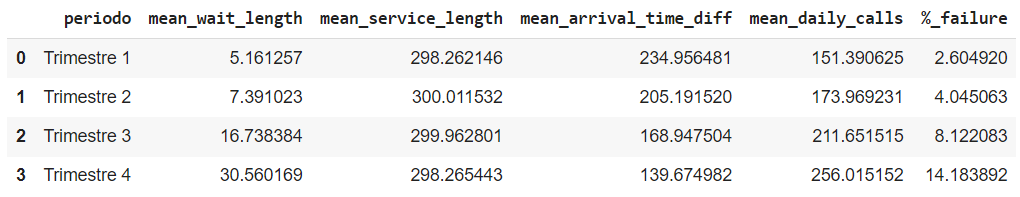
\includegraphics[scale=0.7]{analise-de-dados/trimestral/tritab.png}
    \caption{Tabela de resumo das médias dos tempos de espera, serviço e de chegada de ligações mês a mês}
    \label{fig: tritab_img}
\end{figure}

Tal análise trimestral acaba subestimando a porcentagem de falhas e acaba ocultando algumas informações como a falha no mês de setembro, que está no terceiro trimestre e passa a estar fora da zona de falha estipulada pela gerência.\\
Além disso, também é notável que o caminho correto não é agregar o intervalo de chegadas em períodos ainda maiores, como no trimestre, já que este é um valor alterado mensalmente.\\
Por fim, é possível observar que algumas conclusões semelhantes serão alcançadas em uma análise de cada uma das variáveis, no entanto, há uma perda de informações relevantes, não sendo a melhor maneira de observar o processo.\\